\begin{frame}
   \frametitle{Best-First Search over Paths: Trajectory Optimization}
   \begin{center}
      \includegraphics{build/talk-act1-2d,traja}
      
      \begin{minipage}{0.65\textwidth}
      \begin{algorithmic}
      \Loop
         \State $\Pi \leftarrow $ \textsc{GetPaths}$()$
            \Comment \tikz{\node[draw,circle,inner sep=0.7pt]{\scriptsize 1};}
         \State $\pi^* \leftarrow \argmin\limits_{\pi \in \Pi} f(\pi)$
            \Comment \tikz{\node[draw,circle,inner sep=0.7pt]{\scriptsize 2};}
         \State \textsc{EvalPath}$(\pi^*)$
            \Comment \tikz{\node[draw,circle,inner sep=0.7pt]{\scriptsize 3};}
      \EndLoop
      \end{algorithmic}
      \end{minipage}
   \end{center}
\end{frame}

\begin{frame}
   \frametitle{Best-First Search over Paths: Trajectory Optimization}
   \begin{center}
      \includegraphics{build/talk-act1-2d,trajb}
      
      \begin{minipage}{0.8\textwidth}
      \begin{algorithmic}
      \Loop
         \State $\Pi \leftarrow $ \textsc{GetPaths}$()$
            \Comment Local neighborhood
         \State $\pi^* \leftarrow \argmin\limits_{\pi \in \Pi} f(\pi)$
            \Comment \tikz{\node[draw,circle,inner sep=0.7pt]{\scriptsize 2};}
         \State \textsc{EvalPath}$(\pi^*)$
            \Comment \tikz{\node[draw,circle,inner sep=0.7pt]{\scriptsize 3};}
      \EndLoop
      \end{algorithmic}
      \end{minipage}
   \end{center}
\end{frame}

\begin{frame}
   \frametitle{Best-First Search over Paths: Trajectory Optimization}
   \begin{center}
      \includegraphics{build/talk-act1-2d,trajc}
      
      \begin{minipage}{0.8\textwidth}
      \begin{algorithmic}
      \Loop
         \State $\Pi \leftarrow $ \textsc{GetPaths}$()$
            \Comment Local neighborhood
         \State $\pi^* \leftarrow \argmin\limits_{\pi \in \Pi} f(\pi)$
            \Comment $f(\pi):$ fuzzy approx
         \State \textsc{EvalPath}$(\pi^*)$
            \Comment \tikz{\node[draw,circle,inner sep=0.7pt]{\scriptsize 3};}
      \EndLoop
      \end{algorithmic}
      \end{minipage}
   \end{center}
\end{frame}

\begin{frame}
   \frametitle{Best-First Search over Paths: Trajectory Optimization}
   \begin{center}
      \includegraphics{build/talk-act1-2d,trajd}
      
      \begin{minipage}{0.8\textwidth}
      \begin{algorithmic}
      \Loop
         \State $\Pi \leftarrow $ \textsc{GetPaths}$()$
            \Comment Local neighborhood
         \State $\pi^* \leftarrow \argmin\limits_{\pi \in \Pi} f(\pi)$
            \Comment $f(\pi):$ fuzzy approx
         \State \textsc{EvalPath}$(\pi^*)$
            \Comment Re-linearize
      \EndLoop
      \end{algorithmic}
      \end{minipage}
   \end{center}
\end{frame}

\begin{frame}
   \frametitle{Graph Search: Edge Execution Effort Model}
   \begin{tikzpicture}
   
      \draw[step=1,black!10,very thin,opacity=\gridopacity] (0,0) grid (12,8);
      
      \node[draw,line width=1.0pt,fill=blue!20,minimum width=0.75cm,minimum height=0.10cm]
         (Cfreebox) at (8.0, 7.5) {};
      \node[right=0cm of Cfreebox] {: $\mathcal{C}_{\mbox{\scriptsize free}}$}; 
      
      \node[inner sep=0] at (10.75,7) {%
         \includegraphics[width=2cm]{build/talk-act1-2d,graph}
      };
      
      % bfs
      \only<1>{\fill[green!30] (0.5,5.6) rectangle (5.5,6.9);}
      \only<2>{\fill[green!30] (0.5,5.6) rectangle (5.5,6.15);}
      \only<3>{\fill[green!30] (0.5,6.15) rectangle (5.5,6.9);}
      \node at (2.5,6.75) {\begin{minipage}{5cm}
         \begin{algorithmic}
         \Loop%
            \State $\Pi \leftarrow $ \textsc{GetPaths}$()$
            \State $\pi^* \leftarrow \argmin\limits_{\pi \in \Pi} f(\pi)$
            \State \textsc{EvalPath}$(\pi^*)$
         \EndLoop
         \end{algorithmic}
         \end{minipage}
      };
      
      \only<2>{
         \fill[green!30] (0.1,3.9) rectangle (5.9,4.9);
         \fill[green!30] (6.1,2.5) rectangle (11.9,4.9);
      }
      \only<3>{
         \fill[green!30] (0.1,2.8) rectangle (5.9,3.9);
         \fill[green!30] (6.1,1.6) rectangle (11.9,2.5);
      }
      
      \node[inner sep=0pt,anchor=north] at (3,5.5) {
         \begin{minipage}[t]{5.5cm}%
            \hrule
            \vspace{0.1cm}
            Distance Model $\mathcal{M}_{\ms{dist}}$
            \begin{algorithmic}[1]
            %\only<2-3>{
               \Function {$x_{\ms{\textup{dist}}}$}{$e$}
                  \State \Return $|| q_e(1) - q_e(0) ||$
               \EndFunction
            %}
            \only<3>{
               \Function {$\hat{x}_{\ms{\textup{dist}}}$}{$e$}
                  \State \Return $|| q_e(1) - q_e(0) ||$
               \EndFunction
            }
            \end{algorithmic}
            \hrule
         \end{minipage}%
      };
      
      \node[inner sep=0pt,anchor=north] at (9,5.5) {
         \begin{minipage}[t]{5.5cm}%
            \hrule
            \vspace{0.1cm}
            Set Validity Model $\mathcal{M}_{\ms{valid}}$
            \only<2-3>{
            \begin{algorithmic}[1]
               \Function {$x_{\ms{\textup{valid}}}$}{$e, \mathcal{C}_{\ms{free}}$}
                  \If {${\bf 1}_{\ms{free}}[q_e(t)]$}
                     \State \Return $0$
                  \Else
                     \State \Return $\infty$
                  \EndIf
               \EndFunction
            \only<3>{
               \Function {$\hat{x}_{\ms{\textup{valid}}}$}{$e, \mathcal{C}_{\ms{free}}$}
                  \State \Return $0$
               \EndFunction
            }
            \end{algorithmic}
            }
            \hrule
         \end{minipage}%
      };
      
      \node at (6,0.5) {
         \begin{minipage}[t]{11cm}
         \centering%
         \only<1>{What is the effort model?}%
         \only<2>{Edge evaluation functions (returns execution effort)}%
         \only<3>{Optimistic (admissible) estimates of execution effort}%
         \only<4>{%
         \vspace{-0.4cm}
         \begin{equation*}
            \hat{f}_x(\pi) = \sum_{e \in \pi} \left\{
            \begin{array}{cl}
               x[e] & \mbox{if edge } e \mbox{ evaluated}  \\
               \hat{x}(e) & \mbox{otherwise} \\
            \end{array}
            \right.
         \end{equation*}
         }%
         \end{minipage}
      };
      
   \end{tikzpicture}
\end{frame}

\begin{frame}
   \frametitle{Why Not Just Run A* Graph Search?}
   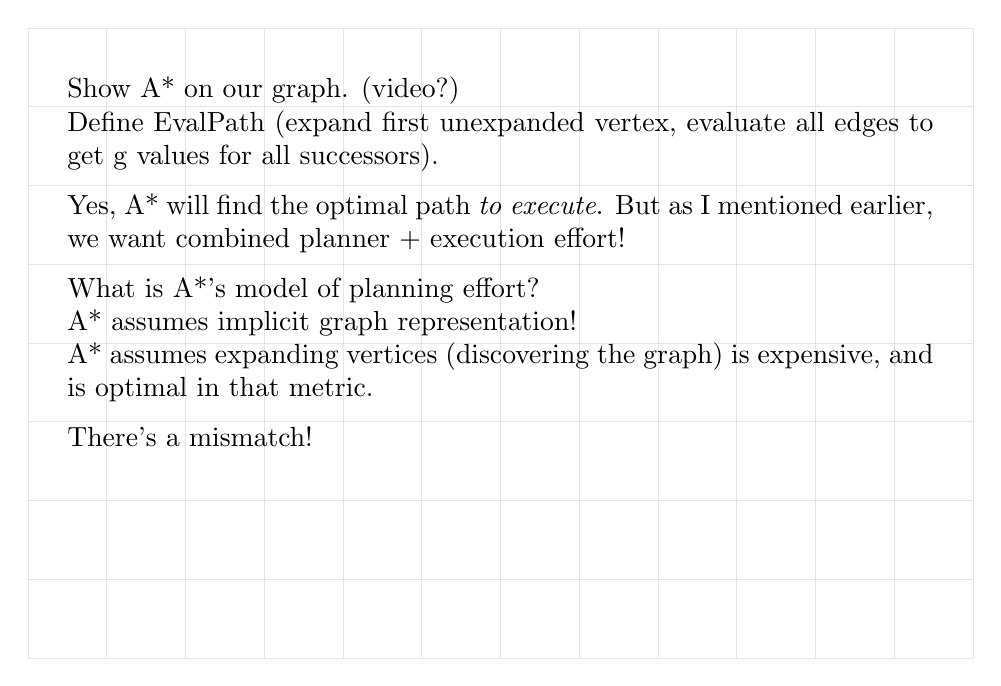
\begin{tikzpicture}
   
      \draw[step=1,black!10,very thin,opacity=\gridopacity] (0,0) grid (12,8);
      
      \node[anchor=north] at (6,7.5)
      {
         \begin{minipage}[t]{11cm}
            Show A* on our graph. (video?)
            
            Define EvalPath (expand first unexpanded vertex,
            evaluate all edges to get g values for all successors).
            
            \medskip
            Yes, A* will find the optimal path \emph{to execute}.
            But as I mentioned earlier, we want combined planner + execution effort!
            
            \medskip
            What is A*'s model of planning effort?
            
            A* assumes implicit graph representation!
            
            A* assumes expanding vertices (discovering the graph)
            is expensive, and is optimal in that metric.
            
            \medskip
            There's a mismatch!
            
         \end{minipage}
      };
      
   \end{tikzpicture}
\end{frame}

\begin{frame}
   \frametitle{Explicit Graph Representation}
   
   Our graphs are small!
   
   Our EvalPath function can be different (e.g. bidirectional).
   Taken from RRTConnect.
   
   Maybe it will perform better?
   
   \begin{equation*}
      \hat{f}_x(\pi) = \sum_{e \in \pi} \left\{
      \begin{array}{cl}
         x[e] & \mbox{if edge } e \mbox{ evaluated}  \\
         \hat{x}(e) & \mbox{otherwise} \\
      \end{array}
      \right.
   \end{equation*}
   
   Similarity to front-to-front algorithms.
   
   This is how Lazy PRM works.
\end{frame}

\begin{frame}
   \frametitle{Roadmaps $\rightarrow$ Graphs}
   \begin{tikzpicture}
   
      \draw[step=1,black!10,very thin,opacity=\gridopacity] (0,0) grid (12,8);
      
      \node[inner sep=0] at (9,5) {%
         {\only<1-4>{\includegraphics{build/talk-act1-2d,graph}}}%
      };
      
      % legend
      \node[draw,line width=1.5pt,fill=blue!20,minimum width=0.75cm,minimum height=0.10cm]
         (Cfreebox) at (3.0, 7.0) {};
      \node[right=0cm of Cfreebox] {: $\mathcal{C}_{\mbox{\scriptsize free}}$}; 
      \node at (3,6.25) {$\Pi$ : set of candidate paths};
      
      \only<1-2>{\fill[green!30] (0.5,3.4) rectangle (5.5,4.1);}
      \only<3>{\fill[green!30] (0.5,2.9) rectangle (5.5,3.4);}
      \only<4>{\fill[green!30] (0.5,3.4) rectangle (5.5,4.1);}
      
      % bfs
      \node at (3,4) {\begin{minipage}{5cm}
         \begin{algorithmic}
         \Loop%
            \State $\Pi \leftarrow $ \textsc{GetPaths}$()$
            \State $\pi^* \leftarrow \argmin\limits_{\pi \in \Pi} f(\pi)$
            \State \textsc{EvalPath}$(\pi^*)$
         \EndLoop
         \end{algorithmic}
         \end{minipage}
      };
      
      \only<2-4>{%
         \node at (6,1) {\begin{minipage}{5cm}%
            \begin{equation*}%
            f(\pi) = {\hat f}_x(\pi) :
            \left\{ \begin{array}{ll}
                x(\pi) & \mbox{if } {\bf 1}_{\mbox{\scriptsize free}}(\pi) \\
                \infty & \mbox{otherwise}
            \end{array} \right.
         \end{equation*}
         \end{minipage}
         };
      }
      
   \end{tikzpicture}
\end{frame}





\begin{frame}
   \frametitle{Best-First Search over Paths: Graphs}
   \begin{center}
      \includegraphics{build/talk-act1-2d,graphfirstnext}
      
      \begin{minipage}{0.65\textwidth}
      \begin{algorithmic}
      \Loop
         \State $\Pi \leftarrow $ \textsc{GetPaths}$()$
            \Comment \tikz{\node[draw,circle,inner sep=0.7pt]{\scriptsize 1};}
         \State $\pi^* \leftarrow \argmin\limits_{\pi \in \Pi} f(\pi)$
            \Comment \tikz{\node[draw,circle,inner sep=0.7pt]{\scriptsize 2};}
         \State \textsc{EvalPath}$(\pi^*)$
            \Comment \tikz{\node[draw,circle,inner sep=0.7pt]{\scriptsize 3};}
      \EndLoop
      \end{algorithmic}
      \end{minipage}
      
      \begin{equation*}
         f_x(\pi) =
         \left\{ \begin{array}{ll}
             x(\pi) & \mbox{if } {\bf 1}_{\mbox{\scriptsize free}}(\pi) \\
             \infty & \mbox{otherwise}
         \end{array} \right.
      \end{equation*}
      
   \end{center}
\end{frame}





\begin{frame}
   \frametitle{Graph Search: Run A*!}
   \begin{tikzpicture}
      \tikzset{>=latex} % arrow heads
   
      \draw[step=1,black!10,very thin,opacity=\gridopacity] (0,0) grid (12,8);
      
      \node[inner sep=0] at (9,5) {%
         {\only<1>{\includegraphics{build/talk-act1-2d,graph}}}%
         {\only<2>{\includegraphics{build/talk-act1-2d,astara}}}%
         {\only<3>{\includegraphics{build/talk-act1-2d,astarb}}}%
         {\only<4>{\includegraphics{build/talk-act1-2d,astarc}}}%
         {\only<5>{\includegraphics{build/talk-act1-2d,astard}}}%
         {\only<6>{\includegraphics{build/talk-act1-2d,astare}}}%
         {\only<7>{\includegraphics{build/talk-act1-2d,astarf}}}%
         {\only<8>{\includegraphics{build/talk-act1-2d,astarg}}}%
         {\only<9>{\includegraphics{build/talk-act1-2d,astarh}}}%
         {\only<10>{\includegraphics{build/talk-act1-2d,astari}}}%
         {\only<11>{\includegraphics{build/talk-act1-2d,astarj}}}%
         {\only<12>{\includegraphics{build/talk-act1-2d,astark}}}%
         {\only<13>{\includegraphics{build/talk-act1-2d,astarl}}}%
         {\only<14>{\includegraphics{build/talk-act1-2d,astarm}}}%
         {\only<15>{\includegraphics{build/talk-act1-2d,astarn}}}%
         {\only<16>{\includegraphics{build/talk-act1-2d,astaro}}}%
         {\only<17>{\includegraphics{build/talk-act1-2d,astarp}}}%
         {\only<18>{\includegraphics{build/talk-act1-2d,astarq}}}%
         {\only<19>{\includegraphics{build/talk-act1-2d,astarr}}}%
         {\only<20-27>{\includegraphics{build/talk-act1-2d,astars}}}%
      };
      
      \node at (3,5.5) {\begin{minipage}{5cm}
         Execution Effort Model:
         \begin{equation*}
            x(e) = \left\{
            \begin{array}{cl}
               ||e|| & \mbox{if } {\bf 1}_{\ms{free}}(e) \\
               \infty & \mbox{otherwise} \\
            \end{array}
            \right.
         \end{equation*}
         Heuristic:
         \begin{equation*}
            {\hat x}(v_a, v_b) = ||v_a - v_b||
         \end{equation*}
         \end{minipage}
      };
      
      \only<21-27>{
         \node at (3,2.25) {Planning Effort Allocation:};
         \draw[] (1,1.5) rectangle (11,2);
      }
      \only<22-27>{
         \draw[fill=yellow] (1.1,1.5) rectangle (1.45,2);
         \node[align=center,inner sep=0] at (0.9,0.8) {\small computing};
         \node[align=center,inner sep=0] at (0.9,0.51) {\small vertex};
         \node[align=center,inner sep=0] at (0.9,0.2) {\small successors};
         \draw[->] (1,1) -- (1.25,1.45);
      }
      \only<23-27>{
         \draw[fill=blue] (1.55,1.5) rectangle (1.95,2);
         \node[align=center,inner sep=0] at (2.8,0.8) {\small sorting};
         \node[align=center,inner sep=0] at (2.8,0.48) {\small open};
         \node[align=center,inner sep=0] at (2.8,0.2) {\small list};
         \draw[->] (2.6,1) -- (1.95,1.45);
      }
      \only<24-27>{
         \draw[fill=red] (2.05,1.5) rectangle (10.9,2);
         \node[align=center,inner sep=0] at (6,0.65) {\small edge};
         \node[align=center,inner sep=0] at (6,0.35) {\small evaluations};
         \draw[->] (6,1) -- (6,1.45);
      }
      
      \only<25-27>{
         \draw[line width=2pt] (1.275,1.75) circle (0.5cm);
      }
      
      \only<26-27>{\node[align=center,fill=white,opacity=0.95] at (7.3,2.9)
         {{\footnotesize Weighted A*}\\{\scriptsize (Pohl 1970)}};}
      \only<27>{\node[align=center,fill=white,opacity=0.95] at (10.2,2.9)
         {{\footnotesize Partial Expansion A*}\\{\scriptsize(Yoshizumi etal. 2000)}};}
      
   \end{tikzpicture}
\end{frame}

\begin{frame}
   \frametitle{Graph Search Mismatch}
   \begin{tikzpicture}
   
      \draw[step=1,black!10,very thin,opacity=\gridopacity] (0,0) grid (12,8);
      
      \node[inner sep=0pt] at (6,7) {\begin{minipage}{12cm}\centering
         A* efficiently addresses {\bf large graphs}, usually represented {\bf implicitly}
         (with {\bf inexpensive edge costs}), by expanding the {\bf fewest vertices}.
      \end{minipage}};
   
      \only<2-4>
      {
         \node[inner sep=0pt] at (2,4.5) {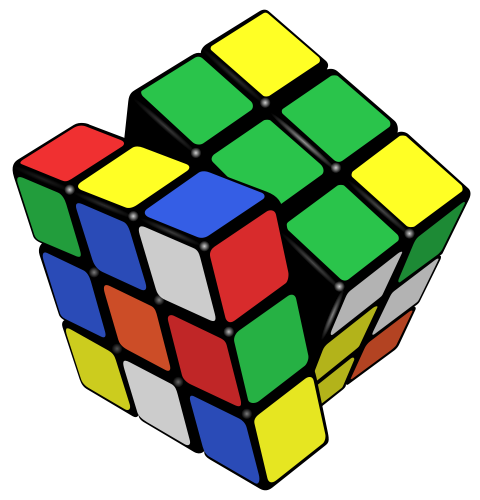
\includegraphics[width=1in]{figs/rubik.png}};
         \node[inner sep=0pt,anchor=north] at (2,2.5)
         {\begin{minipage}{4cm}\centering
            $4.3 \times 10^{19}$ vertices
            
            \tiny{from user Booyabazooka, Wikipedia}
         \end{minipage}};
      }
      
      \only<3-4>
      {
         \node[inner sep=0pt] at (6,4.5) {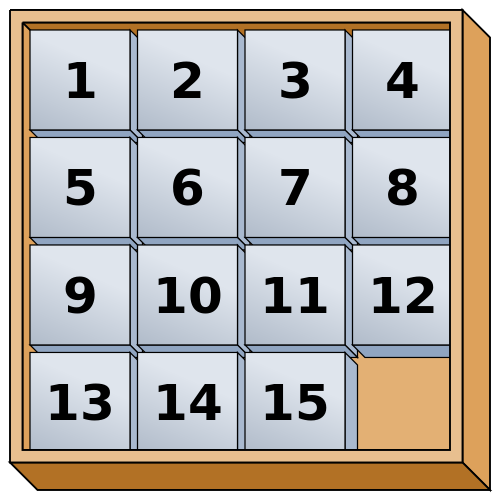
\includegraphics[width=1in]{figs/15puzzle.png}};
         \node[inner sep=0pt,anchor=north] at (6,2.5)
         {\begin{minipage}{4cm}\centering
            $2.1 \times 10^{13}$ vertices
         \end{minipage}};
      }
      
      \only<4>
      {
         \node[inner sep=0pt] at (10,4.5) {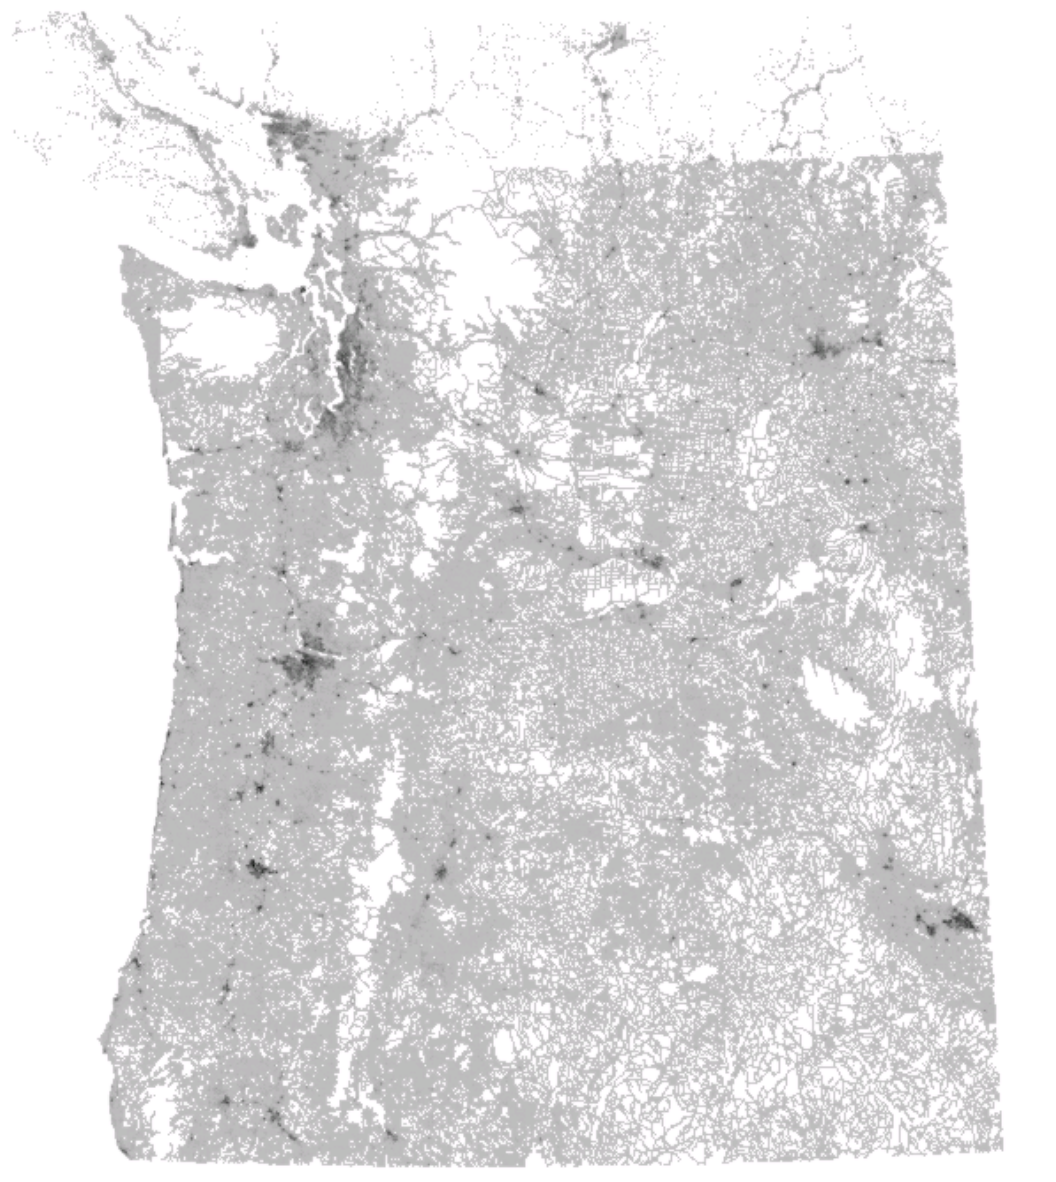
\includegraphics[width=1in]{figs/goldberg-northwest.png}};
         \node[inner sep=0pt,anchor=north] at (10,2.5)
         {\begin{minipage}{4cm}\centering
         
            1.6M vertices
            
            \tiny{
            Goldberg, Harrelson, Kaplan, Werneck.
            ``Efficient Point-to-Point Shortest Path Algorithms''
            }
         \end{minipage}};
      }
   \end{tikzpicture}
\end{frame}

\begin{frame}
   \frametitle{Graph Search Mismatch}
   \begin{tikzpicture}
   
      \draw[step=1,black!10,very thin,opacity=\gridopacity] (0,0) grid (12,8);
      
      \node[inner sep=0pt] at (6,7) {\begin{minipage}{12cm}\centering
         A* efficiently addresses {\bf large graphs}, usually represented {\bf implicitly}
         (with {\bf inexpensive edge costs}), by expanding the {\bf fewest vertices}.
      \end{minipage}};
      
      \only<2-3>{
         \node[inner sep=0pt] at (3.5,4.5) {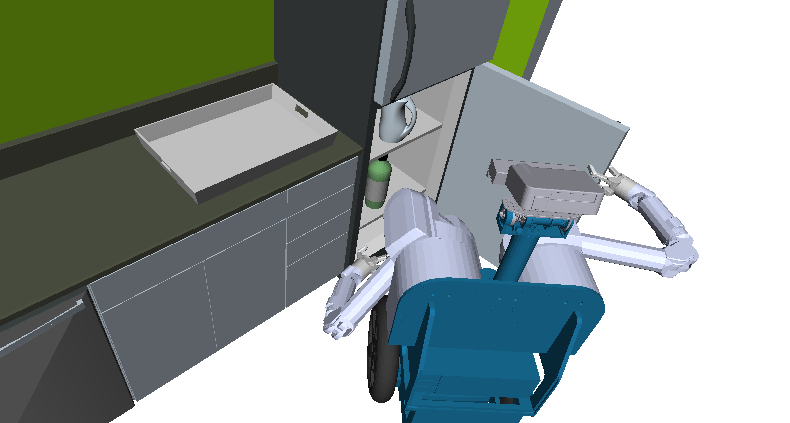
\includegraphics[width=4cm]{figs/fridge-intro.png}};
         \node[inner sep=0pt,anchor=north] at (3.5,3)
         {\begin{minipage}{4cm}\centering
            Our problem:
         
            $\sim10$k vertices
         \end{minipage}};
      }
      
      \only<3>{
         \node[inner sep=0pt] at (8.5,4.5) {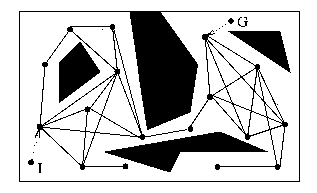
\includegraphics[width=4cm]{figs/prm.png}};
         \node[inner sep=0pt,anchor=north] at (8.5,3)
         {\begin{minipage}{4cm}\centering
            Probabalistic RoadMap
            
            \tiny{Kavraki, Svestka, Latombe, Overmars, 1996}
            
         \end{minipage}};
      }
      
      \only<2-3>{
         \node[inner sep=0pt] at (6,1) {\begin{minipage}{12cm}\centering
            We can represent our graphs {\bf explicitly};
            
            {\bf evaluating graph edges} is expensive,
            
            whereas entire {\bf graph search queries} are inexpensive.
         \end{minipage}};
      }
   
   \end{tikzpicture}
\end{frame}
